\documentclass[a4paper,12pt]{article}

\usepackage[margin=1in]{geometry}
\usepackage[english]{babel}
\usepackage{url}
\usepackage{amsmath,amsthm,amsfonts}
\usepackage{algorithm,algorithmic}
\usepackage[dvips]{color}
\usepackage{wrapfig}
\usepackage{tikz}
\usepackage{tabularx}
\usepackage{booktabs}
\usepackage{colortbl}

\usetikzlibrary{trees}
\usetikzlibrary[positioning]
\usetikzlibrary{calc}
\usetikzlibrary{decorations.pathmorphing}
\usetikzlibrary{fit}
\usetikzlibrary{backgrounds}

\tikzstyle{level 1}=[level distance=4cm, sibling distance=3.5cm]
\tikzstyle{level 2}=[level distance=4cm, sibling distance=2cm]
\tikzstyle{bag} = [text width=4em, text centered]
\tikzstyle{end} = [circle, minimum width=3pt,fill, inner sep=0pt]
\tikzstyle{fork} = [circle, minimum width=3pt,fill, inner sep=0pt]

\title{UROP Progress Report:\\User-centric Webpage Information Extraction}
\date{}
\author{Shawn Tan\\U096883L}
\begin{document}
\bibliographystyle{acm}
\maketitle

\section{Introduction}
Information extraction deals with extracting data from input documents into a structured form. In contrast, information retrieval is concerned with retrieving relevant documents from a collection of documents. Traditionally, the task of information extraction is usually performed on unstructured free text and as such, makes use of certain Natural Language Processing techniques. Web IE however, is concerned with documents extracted from the web. Many of these documents today are in HTML, which are semi-structured, and increasingly, generated by server scripts and template-based. Thus, web information extraction is slightly different from information extraction from free text. In IE, procedures that extract certain information from structured or semi-structured documents like HTML are known as \textit{wrappers}. 

While many systems for web information extraction have been developed over the years, many of these are used in corporate settings, and generally extract huge amounts of data from the web into a form more suited for search and retrieval. While this may be within the reach of corporations, a user who browses the web for leisure does not have access to such resources. Another drawback of these systems is that the process of getting them up and running usually involve many hours of labelling and training work. As a result, these systems are inaccessible to users who do not have the time to do this.
	
The system presented in this report attempts to solve these issues by providing an intuitive interface for labelling that cuts down the amount of annotation required from the user, and also provides a robust information extraction framework by using machine learning to create more robust extraction models.

In the next section, I will discuss previous work done in information extraction and highlight some of the more recent work closely related to ours. In Section 3, a detailed description of the system developed will be given. Section 4 will cover some of the evaluation that has been done with the methods, and Section 5 will conclude the report with future steps that are required.

\section{Related Work}
	Initially, web IE involved manually written wrappers that catered to specific needs and information sources \cite{Chawathe1994,Perkowitz1995} . While this provided accuracy in the information extracted, it required users of the such IE systems to have some background in programming. Later, many wrapper induction tools came about after Kushmerick's paper \cite{Kushmerick1997}, using several different approaches to the problem (e.g. machine learning) \cite{Freitag1998,Soderland}. Subsequently, from 2001, systems that required no user intervention were developed \cite{Chang2001,Crescenzi2002,Arasu2003}. This suggests a trend toward information extraction systems with less human interaction.
	
	However, IE systems cannot completely be free of user intervention. ``Supervised approaches, although require annotation from users, extend well to non-template page extraction if proper features are selected for extraction rules" \cite{Kayed2006}. Since user annotation is crucial to web IE, it is important to improve current user interfaces for labelling. Attempts such as \textit{Lixto}, which has some focus on the user interface aspect of labelling, have tried to make this process more visual \cite{Baumgartner2001}. Other ways to do this would be to reduce the amount of sample data required by the system, or to provide a way to give the user immediate feedback as to what the result of the learnt classifier would be.

	Another problem faced when trying to automate web IE is having to regenerate or re-implement the wrapper every time there is a change in the site layout. This is an important problem given the ease in which templating systems allow pages to be ``themed" and redesigned. Wrappers need to be robust enough to handle such frequent changes, and be less reliant on the underlying HTML structure of the page.
	
	One method of approaching this was to make use of the visual features of the page. The PARCELS system is not strictly an information extraction system, but rather, is concerned with dividing up the page and classifying the resulting blocks correctly. As input, the user is required to input several example pages with labelled blocks as examples. The system then extracts features from 2 different aspects of the blocks: Its \textit{lexical} features and its \textit{stylistic} features. Using both of these the classifier uses a technique called co-training, machine classified blocks from either view is fed into the training data of the other view\cite{Lee2004}. The system was then improved to include usage of inter and intra similarities between pages as features\cite{AikMiang2005}. Gatterbauer also approached the problem of extracting data from web tables by looking directly at the rendered 2D output, extracting tables (or grids) within them, and then analysing these in order to extract relevant information \cite{Gatterbauer2007}.
	
	Dalvi explored the approach of developing a tree-edit model of HTML, modelling changes to a page as a stochastic process, using it to improve wrapper construction for robustness\cite{Dalvi2009}. The method generates a list of candidate XPaths for a certain selected region within the page. It used archived data of a given website to calculate its \textit{compute transformation probability}. Using this, the most robust XPath candidate was selected from the list. This process, however, required access to archives of older versions of the site.

	After studying the drawbacks and advantages of some of the previous work in the area, I hope to make 2 main contributions with my system:
	\begin{enumerate}
		\item Provide an intuitive interface for labelling that is platform agnostic, and takes advantage of the many advancements in Javascript. This will provide the user with an immediate visual feedback as to the items that he/she will be extracting, and at the same time reduce the amount of labelling that needs to be done.
		\item Create a more robust framework for extraction of the selected information using machine learning. The classifier will have less focus on the HTML structural information of the tags in order to be resistant to any layout changes made to the page.
	\end{enumerate}
	For the rest of the paper, I will define users of the system as users who do not have access to resources required by current information extraction system. This includes not only the hardware and processing power required, but also the time needed for the labelling work done. Also, I will define robustness as the wrapper's resistance to changes in HTML structure from the time that the wrapper was derived.
	\chapter{Method}
\label{chap:method}
In the following sections, we will elaborate on the different techniques used in this report.
In the first section we will describe traversal path alignment algorithm, which we
propose to overcome the issues of current methods of XPath generation by providing
a way to create viable XPaths based on elements that users have selected or rejected,
giving them a visual understanding of what will be extracted as they complete the process.

Next, we address the approach we take in trying to create a robust wrapper for the site.
We propose a framework for learning models for classification of HTML tags or DOM nodes by
learning from extracted instances using the XPath.

\input selectioninterface.tex
\input robustextraction.tex


\section{Evaluation}
	At the writing of this report, no formal evaluation of the methods described have been carried out. However, some preliminary tests have been done for several sites, and the results of the methods described in Sections \ref{lcas} and \ref{classificationmodel} look promising.
	
\begin{figure}[htbp]
\centering
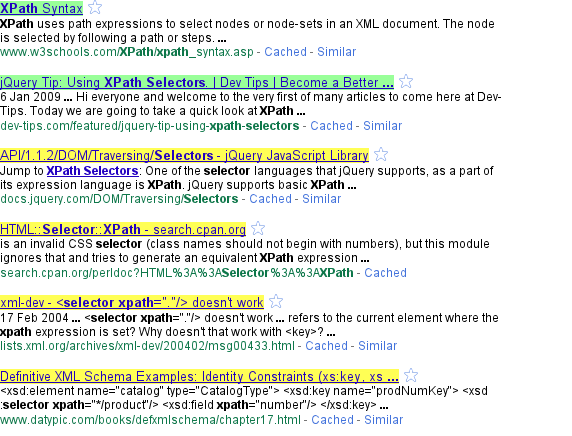
\includegraphics[scale=0.5]{selectorexample.png} 
\caption{User's view when selecting examples}
\label{fig:selectorexample}
\end{figure}
Some tests done using the bookmarklet interface show that the algorithm implemented is quite effective in predicting elements wanted by users. This is especially so when the page in question is highly structured, with many similar repeating elements. This may be due to the strict formatting done when users define a template for their Content Management System, and as a result, class names and attributes for similar elements are consistently reused for headlines, entries etc. Figure \ref{fig:selectorexample} shows the view of the user when selecting items from a Google search result.
\begin{figure}[htbp]
\centering
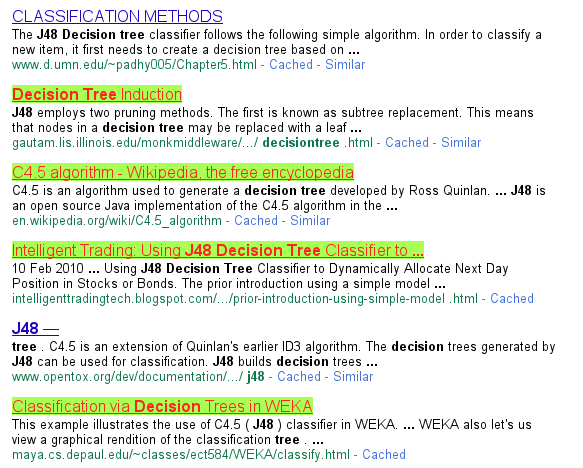
\includegraphics[scale=0.5]{classifierresults.png} 
\caption{User's view when selecting examples}
\label{fig:mlbad}
\end{figure}
The framework used for robust extraction from websites also work well for some sites. On Google search results, the decision tree generated is able to capture most of the entries returned. However, there are some results which do not conform to the constraints specified by the decision tree, and are not selected. This suggests some additional fine tuning must be done to the features extracted. Figure \ref{fig:mlbad} shows 2 items not picked up by the rule.

\section{Future Work \& Conclusion}
The current approach does not solve the issue of unordered elements that are extracted from the pages. While some methods have been devised, none of them have been implemented and tested at this time.

More importantly, in the following semester, more fine tuning of the machine learning component needs to be done. Also, formal evaluation of the methods described has to be carried out.


\bibliography{UROP}{}
\end{document}
